\documentclass{homework}

\usepackage{tcolorbox}
\usepackage{etoolbox}
\usepackage{svg}
\usepackage{algorithm}
\usepackage{algpseudocode}
\usepackage{caption}
\usepackage[newfloat]{minted}
\usepackage{pgfplots}
\usepackage{tabularx}
\pgfplotsset{width=10cm,compat=1.9}
\usepackage[super]{nth}


\begin{document}
\title{Scheduling Project}
\author{32172917 Dabin Lee / 32190984 Isu Kim}
\maketitle

\newminted{python}{frame=lines,framerule=2pt}
\newenvironment{code}{\captionsetup{type=listing}}{}
\SetupFloatingEnvironment{listing}{name=Output or Code}

\maketitle
\begin{center}
Left Free Days : 5
\end{center}
\pagebreak

\section{Index}
\begin{enumerate}
   \item Background Knowledge
   \item Building \& Usage
   \item Round Robin & FIFO Implementation
   \item MLFQ Implementation
   \item Conclusion \& Analysis
   \item References
\end{enumerate}
\pagebreak

\setcounter{section}{0}
\section{Background Knowledge}
In the last task, we studied a multi-programming environment by implementing multi-threads. A scheduling policy is required when selecting a process to assign a processor in multi-programming. Scheduling determines at what point and to which processes are allocated resources alternately used by multiple processes. In this task, we aim to maximize CPU efficiency by implementing and comparing multiple scheduling algorithms after understanding CPU scheduling and looking at performance evaluation criteria.

\subsection{Basic Concepts}
\subsubsection{Preemptive vs Non-preemptive}
\begin{itemize}
    \item \textbf{Non-preemptive Scheduling}: A process keeps the CPU until it releases it either by terminating
    \item \textbf{Preemptive Scheduling}: A process can be preempted by the scheduler.
\end{itemize}

\subsubsection{Decision Making for CPU scheduling}
\begin{figure}[h]
\begin{center}
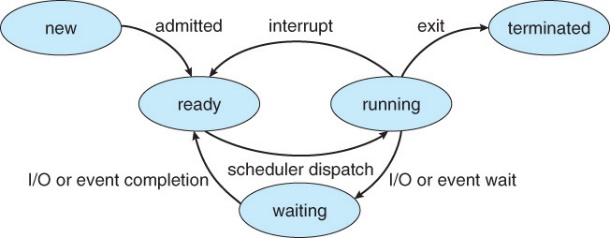
\includegraphics[scale=1.5]{1.png}    
\caption{5 States of a Process}
\end{center}
\end{figure}

\begin{enumerate}
    \item When a process switches from running to waiting state (when calling \texttt{wait()} for the child process to terminate or the result of an I/O request).
    \item When a process switches from running to ready state (when an interrupt occurs).
    \item When a process switches from waiting to ready state (at completion of I/O).
    \item When a process terminates.
\end{enumerate}
In the case of No.1 and No.4, a non-preemptive scheduling policy is used to select a new process after the existing process is executed.
\\
In the case of No.2 and No.3, both preemptive and non-preemptive scheduling policies are available, but we will focus more on preemptive scheduling in future descriptions.
\subsubsection{Scheduling Criteria}
The CPU scheduler schedules the process by considering the following characteristics:
\begin{itemize}
    \item \textbf{CPU utilization}: Keep the CPU as busy as possible.  
    \item \textbf{Throughput}: Number of processes that complete their execution per time unit.
    \item \textbf{Turnaround time}: Amount of time to execute a particular process.
    \item \textbf{Waiting time}: Amount of time a process has been waiting in the ready queue.
    \item \textbf{Response time}: Amount of time it takes from when a request was submitted until the first response is produced.
\end{itemize}

\subsection{CPU Scheduling Algorithms}
The scheduler allocates processors according to the scheduling algorithm and completes the task. There are different kinds of CPU-scheduling algorithms. For intuitive understanding, we describe the main scheduling algorithms based on a single processing core system.

\subsubsection{First-Come, First-Served Scheduling(FCFS)}
The FCFS is the simplest nonpreemptive CPU-scheduling algorithm. In other words, it is called FIFO. As the name suggests, the process that requests the CPU first is allocated the CPU first and it is implemented with a FIFO queue. In this scheduling, when a new process enters the system, the PCB of the process is connected to the end of the ready queue. Then, when it is their turn, the process placed at the front of the ready queue is allocated a processor and leaves the ready queue. To compare and analyze the pros and cons of each scheduling, let's assume CPU burst time of each process. 

\begin{center}
\begin{table}[h]
\begin{tabularx}{1.0\textwidth} { 
  | >{\centering\arraybackslash}X 
  | >{\centering\arraybackslash}X 
  | >{\centering\arraybackslash}X 
  | >{\centering\arraybackslash}X | }
 \hline
 Process & Burst Time\\
 \hline
 P1 & 24\\
 \hline
 P2 & 3\\
 \hline
 P3 & 3\\
\hline
\end{tabularx}
\caption{FCFS Example}
\end{table}
\end{center}
Consider that the arrival time of the following processes is zero and the order of arrival is P1, P2, P3. Then the Gantt chart is drawn as follows:

\begin{figure}[h]
\begin{center}
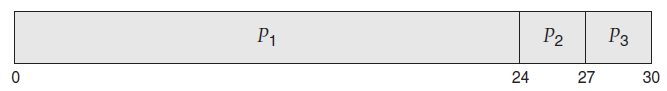
\includegraphics[scale=0.8]{2.png}    
\caption{Gantt Chart of FCFS}
\end{center}
\end{figure}

The average waiting time is $(0 + 24 + 27)/3 = 17$ and the average turnaround time is $(24 + 27 + 30)/3 = 81$, however, if the order of arrival is P2, P3, P1 (Skip the Gantt chart), the average waiting time is now (6 + 0 + 3)/3 = 3 and the average turnaround time is $(3 + 6 + 30)/3 = 13$. In summary, the FCFS policy is simple to implement, but causes worst-case latency by delaying all short jobs after the execution of one long process(convoy effect). So, wouldn't it be the most effective scheduling if we run the shortest tasks in order? This is called \textit{Shortest-Job-First Scheduling(SJF)}. This scheduling can be said to be an optimal algorithm because the average waiting time is intuitively minimized. However, it is basically an unfair scheduling policy because short processes are always set to run first. Also, the most important problem is difficult to implement in practice because it is hard to predict the next process execution time. Therefore, let's continue to look at several different scheduling algorithms to implement SJF scheduling policies as much as possible.

\subsubsection{Priority Scheduling}
Then, it can be thought that the scheduler of the desired results can be completed by introducing the concept of “Priority”. Several factors are considered to calculate the priority, but first, the calculated value is the inverse of the predicted next CPU burst time. That is, the higher the CPU burst time, the lower the priority. Priority scheduling can be preempted or non-preempted. It is a method of assigning a processor to the process with the highest priority by comparing the priority of the newly arrived process with the priority of the process currently running. The main problem with this algorithm is infinite blocking, or starvation. If you are ready to run but high-priority processes continue to come in, low-priority processes have to wait indefinitely. The way to solve this is Aging. Aging is a method of gradually increasing the priority of processes that wait long in a system, and over time, the priority of processes gradually increases.

\subsubsection{Round-Robin Scheduling(RR)}
RR scheduling is preemptive FCFS with a small unit of CPU time. This is called time quantum (or time slice) that is usually 10-100 milliseconds length. It is not very different from FCFS to implement RR scheduling, but if CPU burst of the currently running process is longer than 1 time quantum, that process is preempted and added to the end of the ready queue. Let’s consider that the conditions of CPU burst time and arrival time of each process are the same as FCFS scheduling, and also the order of arrival is P1, P2, P3. Additionally, a time quantum is set to 4 milliseconds. The result of RR is as follows:

\begin{figure}[h]
\begin{center}
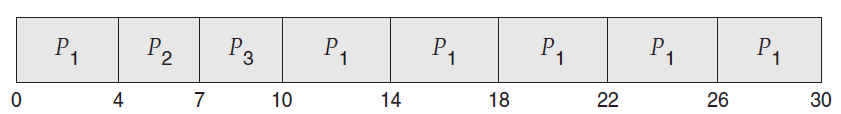
\includegraphics[scale=0.7]{3.png}    
\caption{Gantt Chart of RR}
\end{center}
\end{figure}

\subsubsection{Multilevel Queue Scheduling(MLQ)}
Multilevel queue scheduling is used to divide processes into several separate queues based on the type of process. For example, it can be divided as a foreground(interactive) process and a background(batch) process. Because these two types of processes have different response time requirements, they can have different scheduling requirements. Separate queues might be used for foreground and background processes, and each queue needs its own scheduling algorithm. The foreground queue might be scheduled by an RR algorithm which can provide a high response time to the user and the background queue is scheduled by an FCFS algorithm which focuses on the throughput. In addition, there must be scheduling among the queues. The scheduling methods for this includes \textit{Fixed Priority Scheduling} and \textit{Time Slice Scheduling}. First, for Fixed Priority Scheduling, tasks in the Background Queue wait until tasks in the Foreground Queue are completed. Since it is a fixed priority, low-priority tasks may experience starvation that has to wait for life. Next, the Time Slice Scheduling is a method of distributing the available CPU time for each queue. For example, we can be allocated CPU time that Foreground Queue can be given 80% of CPU time and Background Queue can be given 20% of CPU time.

\subsubsection{Multilevel Feedback Queue Scheduling(MLFQ)}
Since the processes do not change their type of process, so the process should only work in one queue. This has the advantage of relieving the scheduling burden, but has the disadvantage of being less flexible. To address this problem, multi-level feedback queue scheduling has emerged. The MLFQ scheduling algorithm allows a process to move between queues. This is the method to separate processes according to the CPU burst characteristic. If a process uses too much CPU time, it moves to a lower priority queue. This approach leaves I/O bindings and interactive processes, typically characterized by short CPU bursts, in high-priority queues. In addition, processes that wait too long in a low priority queue use aging to solve hunger problems by moving them to a high priority queue. On the other hand, when a process moves to a lower-level queue, the scheduler increases the time quantum for that process, allowing the process to work longer. For example, if a process with a CPU burst time of 35 is processed, it operates as follows:

\begin{figure}[h]
\begin{center}
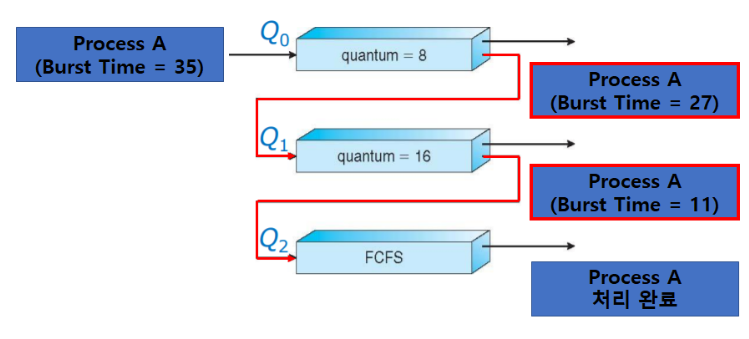
\includegraphics[scale=0.8]{4.png}    
\caption{Example of MLFQ}
\end{center}
\end{figure}


\pagebreak
\section{Building} 
There are 2 directories in this \texttt{git}.
\begin{itemize}
   \item \texttt{rr_fifo}: For implemenation on RR and FIFO
   \item \texttt{mlfq}: For implementation on MLFQ
\end{itemize}

For both \texttt{rr_fifo} and \texttt{mlfq}, there will be a \texttt{Makefile} in the directory. By Using the \texttt{Makefile}, you can compile the project. Each \texttt{Makefile}s include following optional recipes:

\begin{itemize}
   \item \texttt{clean}: For cleaning up object files and compiled program.
   \item \texttt{debug}: For debugging purpose. This will enable \texttt{-DDEBUG} option.
\end{itemize}

For example, if you would like to build RR and FIFO, you can build it by following command.
\\
\begin{center}
\begin{code}
\begin{minted}[frame=single,framesep=10pt]{bash}
$ cd ./rr_fifo
$ make 
\end{minted}
\captionof{listing}{Using \texttt{Makefile} for compiling RR and FIFO}
\end{code}
\end{center}

This will automatically build project and generate an executable file named \texttt{rr_fifo}. Yes, FIFO and RR share the same executable as you might have guessed. For MLFQ, following command will build project.
\\
\begin{center}
\begin{code}
\begin{minted}[frame=single,framesep=10pt]{bash}
$ cd ./mlfq
$ make 
\end{minted}
\captionof{listing}{Using \texttt{Makefile} for compiling MLFQ}
\end{code}
\end{center}

For executing each files, it will be dealt in the later sections.
\pagebreak
\section{Round Robin & FIFO Implementation} 
Since we wanted to mimic how OS schedules each user processes as much as possible, we decided to implement some extra features as well. Those are:
\begin{itemize}
    \item \textbf{IO Burst}: Once a user process finished CPU burst, it will request IO burst to the kernel process.
    \item \textbf{IO Boost}: Once an IO request was finished, the process that issued IO burst will be scheduled right after current running process. However, this IO boost will not refill time quantum.
    \item \textbf{CPU - IO Burst}: Once a user process finished IO burst, it will again go into CPU burst mode. This CPU - IO - CPU - IO ... sequence will be repeated until the user process has its total execution time over.
    \item \textbf{Inactive Queue}: Once a user process had used up all its time quantum, it will be refilled and moved into the inactive queue. Then once the ready queue was empty, the ready queue and inactive queue will be switched automatically.
\end{itemize}
In order for us to implement scheduling along side with extra features, following goals must be achieved:
\begin{enumerate}
    \item \textbf{Process}: Parent process need to create all child processes. Also all child processes and parent process needs to communicate with each other for information, such as IO burst and being scheduled.
    \item \textbf{Scheduling}: Of course, our main goal is to implement an RR scheduling. To save some time implementing FIFO, we decided to use the same code from RR and execute it with very high time quantum which will basically work like a FIFO.
\end{enumerate}
Each goals were achieved by using features from \texttt{C} standard libraries. For communication between each processes, we used message queue and signal for IPC. For Scheduling and time tick passage, we used \textbf{setitimer} for time tick handling. Before we dive deeper into our implementation, in summary, our program operates in following way.
\begin{enumerate}
    \item Initialize message queue using \texttt{msgget}.
    \item Generate user processes using \texttt{fork}.
    \item For user processes, randomly generate CPU burst time and IO burst time. This information is not going to be shared with kernel process.
    \item Kernel process registers timer interrupt handler using \texttt{setitimer}. This will make kernel process know that a time tick passed. Also, time quantum is accounted by kernel process.
    \item Kernel dispatching and stopping a user process will be implemented via signals.
    \item User process requesting IO will be implemented via message queue.
\end{enumerate}
Let us explain how we implemented this project.
\pagebreak

\subsection{Process & Communication}
As we have mentioned before, we use multiple child processes as user process and one parent process as a kernel process. Creating child processes from parent process using \texttt{fork()} is easy. When this program was executed, the parent process will generate 10 child processes using a single \texttt{for} loop. Then each processes will be assigned to work as a child or a parent according to the result value from \texttt{fork}. For example, parent process will call function named \texttt{parent}. Meanwhile child process will call function named \texttt{child}. The implementation of generating multiprocesses can be found under source code in \texttt{rr_fifo/process.c}
\\
In order for those child processes to act properly, we needed some communication between processes. For inter process communication, we considered some various methods. Ranging from sockets to shared memory with semaphore. However, since we thought implementing IPC with shared memory and semaphore will be too painful and will take a long time, we have decided to use signals and message queue for IPC. For other methods, we will try to implement more in the future if we have extra time. So, there shall be two types of communication, which are:
\begin{itemize}
    \item \textbf{Kernel to User}: For dispatching, stopping each user processes and time tick passage.
    \item \textbf{User to Kernel}: For requesting IO.
\end{itemize}
For kernel process to user process communication, we decided to use signals. Since the number of data that kernel process needs to inform user process was limited to 3, signals seemed to be a right fit for this situation. Of course, we might have implemented this via message queue, however we thought signals were better for this type of job. Those signals were defined as it follows:
\label{sec:childSignals}
\begin{itemize}
    \item \texttt{SIGALRM}: For telling user process that a time tick has past. The user process might have accounted for its own time ticks, however this was not the case. As you know, kernel process forks and creates user processes. Which results in kernel process and user process's time tick mismatch. Kernel process will start its time tick faster than user process and this will result in time tick being inaccurately counted.
    \item \texttt{SIGUSR1}: For telling user process that it got CPU time. Consider this as OS kernel dispatching a process. When user process got this signal, it will decrement CPU time when next \texttt{SIGALRM} is received.
    \item \texttt{SIGUSR2}: For telling user process that it now longer has CPU time. Consider this as OS kernel pausing a process. When a user process got this signal, it will no longer decrement CPU time when next \texttt{SIGALRM} is received.     
\end{itemize}
User process has a signal handler that acts upon those signals fired by kernel process. For \texttt{SIGALRM} a function named \texttt{child_timer_handler} was used, and for both \texttt{SIGUSR1} and \texttt{SIGUSR2} a function named \texttt{child_signal_handler} was used. Both signal handlers are implemented under \texttt{rr_fifo/child.c}. 

For user process telling kernel process for IO, signal is not used. Since it needs to send how much IO time was requested, which is normally an \texttt{unsigned int} value, signals were not suitable for this kind of job. Of course we might have implemented it via some methods like \textit{treating \texttt{SIGUSR1} as bit value 0 and \texttt{SIGUSR2} as bit value 1 and combining those as a binary digit information}, however this was just too much. Let's try not to take the hard way while we have some easy way using message queue. There are two types of message queues implemented in this program.
\begin{itemize}
    \item \texttt{up_msg_q}: For telling kernel process that user process is requesting an IO burst. This is named \texttt{up_msg_q} since it is an upstream message queue from user process to kernel process.
    \item \texttt{dn_msg_q}: An downstream message queue from kernel process to user process. However, this is implemented but not used.
\end{itemize}
In every time tick, kernel process will try to retrieve message from message queue using \texttt{msgrcv}. When the message queue was empty, it will consider no IO burst was requested. However, when it receives an message, it will consider current running process requested an IO burst. When the IO burst was recived, kernel thread will make current running process go into wait queue and dispatch next process from the ready queue. We will show you an debug screen on how it works internally.
\\
\begin{center}
\begin{code}
\begin{minted}[frame=single,framesep=10pt]{bash}
...
=============== [ Tick 53 ] ===============
[DEBUG] Sent time tick to child processes 3560398
[DEBUG] Scheduler process received IO request from 3560398 for duration 5 ...
[DEBUG] Moving pid 3560398 to wait queue / IO : 5
[DEBUG] Scheduler dispatching 3560397 in next tick.
[DEBUG] Child 3560398 got SIGUSR2: Stopped
[DEBUG] Child 3560397 got SIGUSR1: Dispatched
[DEBUG] Ready Queue : [3560399|3560400|3560401|3560402]
        Wait Queue : [3560398 : 5]
        Inactive Queue : [3560393|3560394|3560395|3560396]
Running : 3560397
        Remaining Time Quantum : 4

...
\end{minted}
\captionof{listing}{Debug on IPC}
\end{code}
\end{center}
As you can see, in each time tick in kernel process, it will send a \texttt{SIGARM} to user process. When a process got \texttt{SIGUSR1}, it gets dispatched. On the other hand, the process which got \texttt{SIGUSR2} gets stopped. For sending IO request from user process to kernel process, it will put data into the message queue. Also, when user process is sending data to kernel process, it will also send information on if the user process will be finished after this IO burst. 
Now, we are going to explain how this was implemented using pseudo code in the next page.
\pagebreak

First, for each child processes will act upon following pseudo code.
\begin{algorithm}
\caption{Child Process Creation}\label{alg:cap}
\begin{algorithmic}
\State $cpuTime \gets random$
\State $ioTime \gets random$
\State $totalExecutionTime \gets 0$
\State $isRunning \gets False$
\State $isFinished \gets False$
\State register signal handlers for \texttt{SIGUSR1}, \texttt{SIGUSR2}, \texttt{SIGALRM}
\While{!isFinished}  
    \State do nothing
\EndWhile
\State sendIPCMessage() \Comment{For letting scheduler know that this process terminated}
\end{algorithmic}
\end{algorithm}
\\
For signal handling, signal handler was implemented in following way.

\begin{algorithm}
\caption{Child Process Signal Handler for \texttt{SIGUSR1} and \texttt{SIGUSR2}}\label{alg:cap}
\begin{algorithmic}
\If{$signalReceived = \texttt{SIGUSR1}$}
    \State $isRunning \gets True$ \Comment{This means dispatched}
\ElsIf{$signalReceived = \texttt{SIGUSR2}$}
    \State $isRunning \gets False$ \Comment{This means stopped}
\EndIf
\end{algorithmic}
\end{algorithm}

\begin{algorithm}
\caption{Child Process Signal Handler for \texttt{SIGALRM}}\label{alg:cap}
\begin{algorithmic}
\State $totalExecutionTime \gets totalExecutionTime + 1$
\If{$isRunning$ and $!isFinished$} \Comment{CPU was assigned by scheduler}
    \State $cpuTime \gets cpuTime - 1$
\EndIf

\If{$cpuTime <= 0$} \Comment{CPU Burst was over, then request IO Burst}
    \State $isRunning \gets False$
    \If{IO Burst exceeds max execution time}
        \State Use as much IO time available
    \Else
        \State refill $cpuTime$
    \EndIf
    \State Request IO burst to kernel
\EndIf
\end{algorithmic}
\end{algorithm}
\\
For parent process and its signal sending and IPC communication, we will be discussing it in the next section with how scheduling was implemented. Please stay tuned!
\pagebreak

\subsection{Scheduling}
Since our main goal was to implement scheduling simulator, this was one of the most important part that we had to implement. At first, we thought that this will be an easy process, however it turned out to be not the case. 

In order for us to implement scheduling simulator, kernel process needs at least 4 elements to work properly. Those are:

\begin{itemize}
    \item Time tick tracking
    \item Queue managing
    \item Scheduling
    \item IPC
\end{itemize}
Now, let's look into how we implemented elements from now on.

\subsubsection{Time Tick Tracking}
In order for kernel process to know that a time tick has past, keeping track of time ticks were important. Yes, there might have been various ways, such as keeping process in the while loop and calling \texttt{time()} to check how much time has past. However, for us that seemed to be inefficient in terms of it is in a busy waiting state. Therefore, we have decided to use \texttt{setitimer} for tracking time passage. In every time tick, that we have set in the begining of program execution, there will be a \texttt{SIGALRM} fired into the kernel process. With each \texttt{SIGALRM} fired into the kernel process, it will consider a time tick has past. 

As we have mentioned before, the kernel process takes account of all time tick passage. Of course, each user processes might have kept track of time ticks, however due to the difficulty of synchronizing each process's time ticks, we have decided to make kernel process fire \texttt{SIGLARM} into running user process to let it know that a time tick has past. The reason was that if we kept separate time tick handler using \texttt{setitimer}, each processes will start their timer in different moment. This will make time tick tracking in both kernel process and child process having a bit inaccurate result.

\subsubsection{Queue Managing}
In order for kernel process to schedule processes out properly, there should be at least three queues. Those are:

\begin{itemize}
    \item Ready queue
    \item Inactive queue
    \item Wait queue
\end{itemize}

In addition to those queues, we have added another queue that is for terminated processes. This will be used when all the user processes were terminated and scheduler prints out the statistics of each processes.

Queues were implemented using linked list. The reason we picked linked list over arrays or any other implementations were the fact that it will be easier to move each processes around across each queues. Since each processes will be moving around from ready queue to inactive or wait queue, vice versa, we need to keep track of same elements across the queues. Which will be easily implemented via a linked list. Each elements were treated like a PCB. The implementation of PCB in this program was via \texttt{struct}.
\\
\begin{center}
\begin{code}
\begin{minted}[frame=single,framesep=10pt]{c}
struct pcb_t {
    int state;
    pid_t pid;
    unsigned int r_tq;
    struct pcb_t* next;
    unsigned int io_left;
    unsigned long terminated_at;
    unsigned long total_exec_time;
    unsigned long total_io_time;
};
\end{minted}
\captionof{listing}{PCB implementation using \texttt{struct pcb_t}}
\end{code}
\end{center}
We understand implementing queue with linked list is inefficient in terms of time complexity since it needs to find tail of the queue when enqueuing, which is an $O(n)$ operation. However, since the number of processes were limited to 10, this seemed to be compromisable. Also, we had to implement more than just enequeue and dequeue. Those were:
\begin{itemize}
    \item Removing element from the middle of the queue: For IO decrement.
    \item Enqueuing to the head of the queue: For IO boost.
\end{itemize}

If you would like to see how this was actually implemented, you can see following source codes:
\begin{itemize}
    \item \texttt{common.h}: For definition of \texttt{struct pcb_t}.
    \item \texttt{utils.h}: For declaration and definition of each queue related functions.
    \item \texttt{utils.c}: For implementation of each functions declared and defined in \texttt{utils.h}.
\end{itemize}
\subsubsection{Scheduling}
This is the most important part that needs to be implemented. We thought that this would be easier if we explain it with pseudo code. 

\begin{algorithm}
\caption{Parent Process Creation}\label{alg:cap}
\begin{algorithmic}
\State Initialize queues
\State $totalTimeTick \gets 0$
\State Set signal handler for \texttt{SIGALRM} \Comment{By using \texttt{setitimer}}
\State Initialize ready queue with child PIDs
\State $running \gets pop(readyQueue)$ \Comment{Set running process by popping from ready queue}
\State Send signal to $running$ process with signal \texttt{SIGUSR1}
\While{True}
    \State do nothing
\EndWhile
\end{algorithmic}
\end{algorithm}
\pagebreak
Now let's see how the scheduler acts in every time tick.

\begin{algorithm}
\caption{Parent Process \texttt{SIGALRM} handler}\label{alg:cap}
\begin{algorithmic}
\State $totalTimeTick \gets totalTimeTick + 1$
\If {There was running process}
    \State Send signal to $running$ process with \texttt{SIGALRM} \Comment{Let user process know time passage}
    \State $running.totalExecutionTime \gets running.TotalExecutionTime + 1$
    \State $running.remainingTimeQuantum \gets running.remainingTimeQuantum - 1$
    \If {$running.remainingTimeQuantum <= 0$} \Comment{Meaning that time quantum ended}
        \State Send signal to $running$ process with \texttt{SIGUSR2} \Comment{Make user process stop}
        \State Move process into inactive queue
        \State Dispatch next process
    \EndIf
    \State Decrement all IO time in wait queue
    \State Check IPC message queue \Comment{Check if user process issued IO burst}
\Else
    \If{Ready queue was not empty}
        \State $running \gets pop(readyQueue)$
        \State Cancel last time tick event \Comment{This is due to context switching}
        \State Send signal to $running$ process with \texttt{SIGUSR1} \Comment{Make user process start}
    \Else 
        \If{Wait queue was not empty} \Comment{This means all processes are waiting for IO}
            \State Decrement all IO time in wait queue
        \Else \Comment{This means all processes were terminated}
            \State Call exit handler
        \EndIf
    \EndIf
\EndIf
\end{algorithmic}
\end{algorithm}

In short, in every time tick, kernel process will execute following sequence.
\begin{enumerate}
    \item Increment total time tick.
    \item Check running process and perform scheduling if it is necessary.
    \item Decrement all IO time in wait queue.
    \item Check IPC message queue if there was any IO burst request.
    \item Check if all processes were terminated. 
\end{enumerate}
Since putting the whole source code into this document will be too messy, we took important actions from the real source code. If you would like to see how it is implemented in code, please check following source codes (but please be aware of spaghetti codes):
\begin{itemize}
    \item \texttt{parent.h}: For declaration and definition of each scheduling related functions.
    \item \texttt{parent.c}: For implementation of each functions declared and defined in \texttt{parent.h}.
\end{itemize}
\pagebreak

For dispatching next process, it is executed with following pseudo code:
\begin{algorithm}
\caption{Scheduler Dispatcher}\label{alg:cap}
\begin{algorithmic}
    \State $running \gets pop(readyQueue)$
    \If{$running == NULL$} \Comment{Meaning that current ready queue was empty}
        \State Swap ready queue and inactive queue
        \State $running \gets pop(readyQueue)$
        \If{$running == NULL$} \Comment{This means all processes were terminated}
            \State Call exit handler
        \Else
            \State Send signal to $running$ process with \texttt{SIGUSR1} \Comment{Make user process start}
        \EndIf
    \Else
        \State Send signal to $running$ process with \texttt{SIGUSR1} \Comment{Make user process start}
    \EndIf
\end{algorithmic}
\end{algorithm}

This will make it possible for parent process which works as an kernel process able to perform scheduling based upon round robin scheduling. 

\subsubsection{IPC}
For inter process communication between kernel process and user process, signals and message queues were used. Signals are used to inform user process know that they are being dispatched or being stopped. Those are achived by two signals \texttt{SIGUSR1} and \texttt{SIGUSR2}. Please check \hyperref[sec:childSignals]{here} for more information on how child receives signals and how it acts upon each signals.

Each user processes will send data through message queues when they are requesting IO burst or they have been executed more than their maximum execution time. The message queue will be delivered in a form of \texttt{struct}. 
\\
\begin{center}
\begin{code}
\begin{minted}[frame=single,framesep=10pt]{c}
struct msg_q_data_t {
    int mtype; 
    pid_t pid;
    unsigned int io_request;
    int is_finished;
};
\end{minted}
\captionof{listing}{Message Queue using \texttt{struct msg_q_data_t}}
\end{code}
\end{center}

The data will be delivered from child process using \texttt{msgsnd} and will be received by parent process using \texttt{msgget}. This program also deletes message queue using \texttt{msgctl} to remove unnecessary message queue leftovers which might affect next execution. By those four elements from 3.2.1 to 3.2.4, we can achieve implementing scheduling.

\pagebreak
\subsection{Execution}
In order to execute this program, you need to first compile the project. Please refer to Section 2. for more information on how to build this project.


You can execute \texttt{rr_fifo} using following command.
\\
\begin{center}
\begin{code}
\begin{minted}[frame=single,framesep=10pt]{bash}
$ ./rr_fifo <time_quantum> <time_tick>
\end{minted}
\captionof{listing}{Executing \texttt{rr_fifo}}
\end{code}
\end{center}
\\
\texttt{rr_fifo} supports two commandline arguments:
\begin{itemize}
   \item \texttt{time_quantum}: For determining how much time ticks for a time quantum.
   \item \texttt{time_tick}: For determining interval of each time ticks in millisecond.
\end{itemize}
\\
So, an example execution command will be as it follows:
\\
\begin{center}
\begin{code}
\begin{minted}[frame=single,framesep=10pt]{bash}
$ ./rr_fifo 10 30
\end{minted}
\captionof{listing}{Example executing \texttt{rr_fifo}}
\end{code}
\end{center}
\\
This will make RR scheduling with 30ms time tick interval with 10 time ticks per time quantum. Please be ware that using time tick that is too small might have inaccurate results. This is one of the limitations of this program and will be dealt in later section.
\\
\begin{center}
\begin{code}
\begin{minted}[frame=single,framesep=10pt]{bash}
[+] Initialized queues.
----------=[ Scheduler ]=----------
[+] Starting job...
    Time Quantum : 10 time ticks
    Time Tick : 50 ms
    Output file : schedule_dump.txt
[+] Child 0 generated with PID 3637332
[+] Child 1 generated with PID 3637333
...
[+] Child 7 generated with PID 3637339
[+] Starting scheduling in 1 second.
[+] Child 8 generated with PID 3637340
[+] Child 9 generated with PID 3637341
\end{minted}
\captionof{listing}{Example executing \texttt{rr_fifo}}
\end{code}
\end{center}
\\
After this output, the scheduling will begin. It will iterate until each user processes hit maximum execution time. The maximum execution time of each child processes are defined in \texttt{child.h} as \texttt{CHILD_MAX_EXECUTION_TIME}. By default, it is set to 50 time ticks for each user processes.

Also the execution result will be written in a file named \texttt{schedule_dump.txt} in the same directory that \texttt{rr_fifo} executable file resides in. It will store results in following format:
\\
\begin{center}
\begin{code}
\begin{minted}[frame=single,framesep=10pt]{bash}
$ cat ./schedule_dump.txt
=============== [ Tick 2 ] ===============
Ready Queue : [3637731|3637732|3637733|3637734|3637735|3637736|3637737|...
        Wait Queue : []
        Inactive Queue : []
Running : 3637730
        Remaining Time Quantum : 9
...
\end{minted}
\captionof{listing}{Example output of \texttt{schedule_dump.txt}}
\end{code}
\end{center}
\\
Once the program finished execution, it will print out an statistics on each processes. Those statistics include following information:

\begin{itemize}
    \item Execution time: The total time that this process used CPU.
    \item Turn around time: The turn around time.
    \item IO time: The total time that this process requested IO burst.
    \item Wait time: The total time that this process was in ready queue. The name is quite confusing since it is in ready queue but treated as a waiting time. But please understand our poor choice of word.
\end{itemize}

Once statistics of each processes were printed out, it will print out average information. This looks something like this:
\\
\begin{center}
\begin{code}
\begin{minted}[frame=single,framesep=10pt]{bash}
[Scheduler] All processes were terminated.
[Scheduler] Killing all child processes..
[Scheduler] Sending SIGKILL to child 3638484
...
=============== [Stats] ===============
PID: 3638488
     Execution Time : 26
     IO Time : 21
     Turn around time : 237
     Wait time: 190
PID: 3638484
     Execution Time : 33
     IO Time : 21
     Turn around time : 276
     Wait time: 222
...
Average turn around time : 289
Average wait time : 238
[+] Destroyed queues.
\end{minted}
\captionof{listing}{Example output statistics}
\end{code}
\end{center}
\\
\pagebreak
Also, you can stop execution of the program by using \texttt{SIGINT} if you would like to stop program while it is being executed. Please use \texttt{CTRL + C} or \texttt{kill} to send signal to the kernel process. Once the kernel process gets \texttt{SIGINT}, it will automatically send \texttt{SIGKILL} to all child processes. 

We have tested the feature of cleaning up the child processes by killing parent process, however in order for you to be extra cautious, please check if all processes were terminated properly. For example, you can use \texttt{top}, \texttt{htop}, \texttt{ps -ef | grep rr_fifo} for checking if all processes were terminated. If not, please kill them using \texttt{kill} or \texttt{pkill}. We tried not to make a fork bomb, however there were some cases that actually happened in the local machine. So, please be extra careful when exiting the program.

\subsection{Analysis}
\label{sec:rrconclusion}

With different time quantum durations, we can compare FIFO and RR's scheduling performance. Since we have learned them in the class time, let's check how these actually behave. We set all CPU burst time and IO burst time as 5 time ticks for each user processes. Also, we are assuming all processes have arrived at the queue at the same time. All user processes will execute for 50 time tick and finish execution.

\subsubsection{Time Quantum 1}
If we set time quantum as 1 time tick, we had following result.

\begin{center}
\begin{table}[h]
\begin{tabularx}{1.0\textwidth} { 
  | >{\centering\arraybackslash}X 
  | >{\centering\arraybackslash}X | }
 \hline
 AVG Turn Around Time & AVG Wait Time\\
 \hline
 2828 & 2539\\
\hline
\end{tabularx}
\caption{Time Quantum as 1}
\end{table}
\end{center}

Also, each processes finished in a very close time with each other. Meaning that using small time quantum makes all processes end almost at the same.

\subsubsection{Time Quantum 4}
Since each user process uses 5 time ticks, we are giving a time quantum that is lower than actual CPU burst time. Meaning that this will make each user processes to take at least 2 time quantum to finish their CPU burst and request IO burst. The result was as it follows.

\begin{center}
\begin{table}[h]
\begin{tabularx}{1.0\textwidth} { 
  | >{\centering\arraybackslash}X 
  | >{\centering\arraybackslash}X | }
 \hline
 AVG Turn Around Time & AVG Wait Time\\
 \hline
 331 & 276\\
\hline
\end{tabularx}
\caption{Time Quantum as 4}
\end{table}
\end{center}

\subsubsection{Time Quantum 100 (FIFO)}
We gave each process an unlimited time ticks. Since each processes take up 50 maximum time ticks, giving 100 time ticks as time quantum will make scheduling work like a FIFO scheduler. With FIFO scheduling, the result was as it follows.

\begin{center}
\begin{table}[h]
\begin{tabularx}{1.0\textwidth} { 
  | >{\centering\arraybackslash}X 
  | >{\centering\arraybackslash}X | }
 \hline
 AVG Turn Around Time & AVG Wait Time\\
 \hline
 169 & 111\\
\hline
\end{tabularx}
\caption{Time Quantum as 100 (FIFO)}
\end{table}
\end{center}

So as it is like in the textbook, we can know following information:
\begin{itemize}
    \item \textbf{Big Time Quantum}: Will perform just like FIFO, having better turn around time and better wait time.
    \item \textbf{Small Time Quantum}: Will make turn around time and wait time painful.
\end{itemize}

Let's investigate why this happens in simple math. This is an equation that we have derived, therefore it might be totally off. 

Assumption is as it follows
\begin{itemize}
    \item All jobs arrived at the same time.
    \item All jobs have same execution time.
    \item Job $i$ is $i$th from head of the ready queue.
\end{itemize}

Let $t$ as total execution time of process. Also let's say we have $n$ processes. Time quantum was given as $tq$. With those information we can derive following formula:

\[
    turnaround_i = \frac{t}{tq} * n + i
\]

For getting average of turn around time, we can use following formula:

\[
    avgTurnAround = \frac{\sum_{i=1}^{n}turnaround_i}{n} = \frac{\sum_{i=1}^{n}\{\frac{t}{tq}*n + i\}}{n} = \sum_{i=1}^{n}\frac{t}{tq} + \frac{n}{(n+1)*n} = \sum_{i=1}^{n}\frac{t}{tq} + \frac{1}{n+1} 
\]

Simply speaking, $\frac{1}{n+1}$ is not controllable, which can be regarded as a constant value. Meanwhile, if we have large $tq$, that will make $\sum_{i=1}^{n}\frac{t}{tq}$ bigger. Resulting bigger turn around time. Also for average waiting time, waiting time can be calculate as following formula:

\[
    wait_i = turnaround_i - t
\]
Therefore, turn around time also affects wait time. Meaning that if we have a higher $tq$, that will result bigger turn around time. Bigger turn around time will make wait time bigger. Therefore making the average waiting time bigger.
\\
Of course this is just an assumed case. However, we can get a glimpse of how time quantum can affect total performance of scheduling. In short, bigger time quantum will make turn around and wait time smaller. In the mean time, with smaller time quantum, time quantum and wait time gets bigger.

\pagebreak

\subsection{Limitations}
There is a list of limitations with this program. Those limitations are due to technical difficulties and lack of experience in programming. The list below is a list of found limitations till now in our environment:

\begin{itemize}
    \item \textbf{Fork bomb}: We have implemented a signal handler with parent process that kills all child processes when parent process finished execution. However, if the parent process was not terminated properly, such as segmentation fault during runtime and killing process with \texttt{SIGTSTP}, the child processes might become zombie processes. Therefore, please check if all child processes were terminated successfully with some basic Linux commands.
    \item \textbf{Dispatch delay}: When there was no running process and scheduler dispatches next process from ready queue. There is a tick delay between scheduler dispatching next process and when it is actually getting dispatched and uses CPU time. Please just consider this issue as an context switch in multiplexing processes.
    \item \textbf{Time tick}: When the time tick interval is defined with a small value, such as 10ms, there is high chance of tick getting inaccurately counted. This is due to the kernel's time tick being faster than the actual user process processing that time tick event. For example, let's suppose that you set time tick interval as 1ms and user process takes 5ms to process each time ticks fired by kernel process, there will be a potential of user process skipping time tick. For example, it might decrement CPU burst time more than it should and the burst time might hit negative number. Therefore use a time tick which is more than 10ms.
    \item \textbf{Max execution time}: Due to the random numbers that user process generate, the maximum execution time of each user process will not be hard limited to the maximum execution time. Please consider maximum execution time of each user processes set by \texttt{CHILD_MAX_EXECUTION_TIME} as an soft limit of each user process's execution time.
    \item \textbf{Random numbers}: When the parent process \texttt{fork}s, each child processes generate random numbers for CPU burst and IO burst duration. However, since the random is based upon a seed that depends solely on the time, there might high chances of multiple user process having same CPU burst and same IO burst duration. 
\end{itemize}

Those are known limitations and bugs that were discovered till now with this program. There might be more bugs in the program other than those listed above, please keep an eye on this program when it is being executed. 
\pagebreak
\section{MLFQ Implementation} 
Before we start MLFQ implementation, there is a famous quote that we would like to share.

\makeatletter
\newenvironment{chapquote}[2][2em]
  {\setlength{\@tempdima}{#1}%
   \def\chapquote@author{#2}%
   \parshape 1 \@tempdima \dimexpr\textwidth-2\@tempdima\relax%
   \itshape}
  {\par\normalfont\hfill--\ \chapquote@author\hspace*{\@tempdima}\par\bigskip}
\makeatother
\begin{chapquote}{Edsger W. Dijkstra}
``If debugging is the process of removing software bugs, then programming must be the process of putting them in.''
\end{chapquote}

We are going to put some more bug into the program by implementing MLFQ. Actually there were some options of implementing besides MLFQ. Those were:

\begin{itemize}
    \item \textbf{CFS (Completely Fair Scheduler)} $O(1)$ Scheduler: Since Linux is currently using this. 
    \item \textbf{BFS (Brain Fuck Scheduler)} $O(N)$ Scheduler: Since the name was interesting. This is not implemented via \texttt{Brainfuck} language unfortunately though. 
\end{itemize}
However, we picked MLFQ since this looked more fun to implement. Also, MLFQ seemed to have more reusable code that we have written so far. So we choose MLFQ over other schedulers. If we have any free time in the future, we will be implementing BFS, since the name is interesting. 

Before we start implementing MLFQ, let's quickly remind rules of MLFQ. We are going to use the improved MLFQ with 5 rules.
\begin{enumerate}
    \item If \texttt{Priority(A)} > \texttt{Priority(B)}, $A$ runs, $B$ doesn't.
    \item If \texttt{Priority(A)} = \texttt{Priority(B)}, $A$ \& b $B$ runs in RR.
    \item When job enters the system, it is placed at the highest priority.
    \item Once a job uses up its time allotment at a given level (regardless of how many times it has given up CPU), its priority is reduced.
    \item After some time period S, move all the jobs in the system to the topmost queue.
\end{enumerate}
For ease of implementation, we are going to modify a bit of rules from MLFQ.
\begin{enumerate}
    \item No change
    \item No change
    \item No extra jobs enter the system. When our scheduler simulator starts, it will place all processes in random queue levels. We could have implemented new job registration, however that would make \texttt{fork} sequence from parent process a bit more complicated.
    \item Assume "time allotment" as "time quantum". Therefore, we are going to reduce priority when a job uses up its all time quantum.
    \item Kernel process will account for all waiting time of processes. When a process takes CPU time, the waiting time will be reset to 0. If that waiting time reaches some value $S$, that process will be promoted to the topmost queue. This is to Avoid all processes going into the topmost queue. Which will make MLFQ act like a RR scheduler.
\end{enumerate}
Modifying the rules will have make the scheduling quite apart from MLFQ. However, those rules were changed due to ease of implementation and for better demonstration. So, please understand our rude modification.
\pagebreak
In order for us to implement (slightly modified) MLFQ, following goals must be achieved:
\begin{itemize}
    \item \textbf{Multiple Queues}: Of course, as its name implies, it needs multiple queue implementation.
    \item \textbf{Priority Boost}: After some time $S$, we need to make the process go into the topmost queue. This is from \textit{Rule 5.}
\end{itemize}
\subsection{Slight Modification}
Luckily, we have a portion of code that we can reuse! Let's try not to reinvent the wheel.

In order for us to perform "priority boost", we need to store how much this process has been not using CPU. Also, to make a process go back to the queue where it was after IO burst, the queue where it came from must be stored as well. Therefore, we need to modify a bit of \texttt{struct pcb_t} to store additional information.
\\
\begin{center}
\begin{code}
\begin{minted}[frame=single,framesep=10pt]{c}
struct pcb_t {
    int state; 
    pid_t pid; 
    int queue_stat; // Store where this process was!
    unsigned int r_tq;
    struct pcb_t* next; 
    unsigned int io_left; 
    unsigned long registered_at;
    unsigned long terminated_at; 
    unsigned long total_exec_time; 
    unsigned long total_io_time;
    unsigned long wait_time; // Store how much this process starved.
};
\end{minted}
\captionof{listing}{PCB implementation using \texttt{struct pcb_t}}
\end{code}
\end{center}

With this slight modification, and some other modification, we could reuse legacy code from RR and FIFO implementation. If you would like to see how each code was changed and modified, please take a look at our source code. 

\subsection{Multiple Queues}
Since this is a multi level queue, we need to implement multiple queues. Implementing multiple queues was not a difficult process since we already have implemented queues in RR and FIFO implementation with linked list. We need at least three queues to implement MLFQ.
\begin{itemize}
    \item \textbf{Wait Queue}: For processes which are waiting for IO jobs.
    \item \textbf{Terminated Queue}: For processes which got terminated. This is for statistics only.
    \item \textbf{Level Queues}: For storing each levels of queues.
\end{itemize}

Implementing multiple queues was not a difficult process. However, managing the queues between level queues were a bit tricky. In more detail, for level queues, we need following features:
\begin{itemize}
    \item \textbf{Demoting}: For moving process to the lower queue.
    \item \textbf{Promoting}: For moving process to the upper queue.
    \item \textbf{IO Restore}: When a process finished IO burst, the process needs to be put back to the queue where it was at. At here, we do not refill time quantum due to the Rule 4. 
    \item \textbf{Priority Comparison}: In every time tick, we need to check if there was any higher priority process in all queue levels. If there was a higher priority process, stop current running process and dispatch higher priority process immediately. This happens due to priority boost. For example, current running process was at level 3, and a process at level 4 was priority boosted then moved into the topmost queue. In this situation, current running process will be scheduled out and priority boosted one will be dispatched.
\end{itemize}

Priority comparison can be expressed as following pseudo code.
\begin{algorithm}
\caption{Priority Comparison}\label{alg:cap}
\begin{algorithmic}
\State $beforeQueue \gets currentSelectedQueue$
\For{$i \gets 0$ to $queueCount$} \Comment{Iterate over all queue levels.}
    \If{Queue $i$ is not empty and $i$ has higher priority}
        \State $currentSelectedQueue \gets i$
    \EndIf
\EndFor
\If {$beforeQueue != currentSelectedQueue$}
    \State Stop current running process.
    \State Push running process back to the queue.
    \State $running \gets Queue[currentSelectedQueue].pop$
    \State Refill $running$ process and dispatch.
\EndIf
\end{algorithmic}
\end{algorithm}
The implementation of this code can be found as \texttt{update_queue_stats()} under \texttt{mlfq/parent.c}. After implementing priority comparison and queue level scheduling, we pretty much implemented most out of MLFQ. For priority boost and all other features, those are obvious functions. Thus, we will skip detailed description on implementation. If you would like to see how each features are implemented in the code, please check following functions under \texttt{mlfq/parent.c}. The file has detailed comments and fucnction documentations, so it will be easy to track flow of each functions.
\begin{itemize}
    \item \texttt{dispatch_next()}: For dispatching next process.
    \item \texttt{time_quantum_over()}: For taking care of running process getting time quantum expired.
    \item \texttt{perform_priority_boost()}: For performing priority boost. Implementation of Rule 5.
    \item \texttt{update_queue_stats()}: For updating queues and comparing queue priorities. 
\end{itemize}
In short, implementing MLFQ was easy. It just required a bit of modification in scheduling algorithm. IPC and all other features were reused.
\pagebreak
\subsection{Execution}
In order to execute this program, you need to first compile the project. Please refer to Section 2. for more information on how to build this project.


You can execute \texttt{mlfq} using following command.
\\
\begin{center}
\begin{code}
\begin{minted}[frame=single,framesep=10pt]{bash}
$ ./mlfq <number of levels> <time_tick>
\end{minted}
\captionof{listing}{Executing \texttt{mlfq}}
\end{code}
\end{center}
\\
\texttt{mlfq} supports two commandline arguments:
\begin{itemize}
   \item \texttt{number_of_queues}: For determining how many levels of queues to generate.
   \item \texttt{time_tick}: For determining interval of each time ticks in millisecond.
\end{itemize}
\\
So, an example execution command will be as it follows:
\\
\begin{center}
\begin{code}
\begin{minted}[frame=single,framesep=10pt]{bash}
$ ./mlfq 5 30
\end{minted}
\captionof{listing}{Example executing \texttt{mlfq}}
\end{code}
\end{center}
\\
This will make 5 levels of queues with each time tick as 10ms interval. As level increases, each level will have 5 time tick jump for their time quantum. For example, level 0 will have 5 time ticks as a time quantum. Then with level 1, it will be 10, with level 2, it will be 15. The number of how much each time ticks will be increased can be defined as \texttt{TIME_TICK_JUMP} under \texttt{mlfq/parent.h}. Also, the $S$ value that determines each priority boost can be determined with \texttt{S} under \texttt{mlfq/parent.h} as well. 

After the program gets started, it will assign 9 processes into random queues. One process will be assigned at the topmost queue. An example execution output will be like below.
\\
\begin{center}
\begin{code}
\begin{minted}[frame=single,framesep=10pt]{bash}
----------=[ Scheduler ]=----------
[+] Initializing queues.
[+] Initialized queues.
[+] Starting job...
    Total Queue count : 5
    Output file : schedule_dump.txt
[+] Child 0 generated with PID 3882089
...
- Level 0 : Time Quantum 5
- Level 1 : Time Quantum 10
- Level 2 : Time Quantum 15
- Level 3 : Time Quantum 20
- Level 4 : Time Quantum 25
...
\end{minted}
\captionof{listing}{Example executing \texttt{mlfq}}
\end{code}
\end{center}
\pagebreak
If you have \texttt{DEBUG} option enabled, it will show more detailed status of each queues with detailed information. In order to set \texttt{DEBUG} option, you can build the project with \texttt{make debug} instead of original recipe. An example output is like below.
\\
\begin{center}
\begin{code}
\begin{minted}[frame=single,framesep=10pt]{bash}
...
[DEBUG] Child 3882089 got SIGUSR1: Dispatched
=============== [ Tick 1 ] ===============
[>] Level 0: [3882095|3882096|3882098] (3)
[ ] Level 1: [3882090|3882092|3882094] (3)
[ ] Level 2: [3882093|3882097] (2)
[ ] Level 3: [3882091] (1)
[ ] Level 4: [] (0)
Current Level : 0
Wait Queue: [] (0)
Running : 3882089 (4)
[DEBUG] Child 3882089 Timer Ticked! : Total Time Tick 1 / Is running 1 / ...
...
\end{minted}
\captionof{listing}{Example executing \texttt{mlfq}}
\end{code}
\end{center}

When the program executes, it will also generate a log file on scheduling dump. This will be logged until 10,000 time ticks. This file will be named as \texttt{schedule_dump.txt} which can be found in the same directory as the executable file. An example schedule dump is like below.
\\
\begin{center}
\begin{code}
\begin{minted}[frame=single,framesep=10pt]{bash}
...
=============== [ Tick 1 ] ===============
[>] Level 0: [3882330] (1)
[ ] Level 1: [3882324] (1)
[ ] Level 2: [3882326] (1)
[ ] Level 3: [3882323|3882325|3882328] (3)
[ ] Level 4: [3882327|3882329|3882331] (3)
Current Level : 0
Wait Queue: [] (0)
Running : 3882322 (4)
...
\end{minted}
\captionof{listing}{Example of \texttt{schedule_dump.txt}}
\end{code}
\end{center}
When the process terminates successfully after all the user processes finished execution, it will print out the statistics. Also, if you would like to terminate \texttt{mlfq} process while executing, please use \texttt{CTRL + C} to send \texttt{SIGINT}. An example statistics will be shown like below:
\pagebreak
\begin{center}
\begin{code}
\begin{minted}[frame=single,framesep=10pt]{bash}
...
=============== [Stats] ===============
PID: 3882322
     Execution Time : 32
...
Average turn around time : 218
Average wait time : 172
[+] Destroyed queues.
\end{minted}
\captionof{listing}{Example of Statistics}
\end{code}
\end{center}
\label{sec:mlfqconclusion}

\subsection{Analysis}
After executing \texttt{mlfq} multiple times with different settings, we found some results and scheduling operations which we found it interesting. If we set $S$ as 50 time ticks and \texttt{TIME_TICK_JUMP} with 5 queues, in some time following result occurs.
\\
\begin{center}
\begin{code}
\begin{minted}[frame=single,framesep=10pt]{bash}
...
=============== [ Tick 174 ] ===============
[ ] Level 0: [] (0)
[>] Level 1: [3883280|3883272|3883274|3883273|3883278|3883276|3883279|...] (9)
[ ] Level 2: [] (0)
[ ] Level 3: [] (0)
[ ] Level 4: [] (0)
Current Level : 1
Wait Queue: [] (0)
[DEBUG] Scheduler process received IO request from 3883281 for duration 5 ...
[DEBUG] Moving pid 3883281 to wait queue / IO : 5
Running : 3883280 (10)
[DEBUG] Child 3883281 got SIGUSR2: Stopped
[DEBUG] Child 3883280 got SIGUSR1: Dispatched
...
\end{minted}
\captionof{listing}{Interesting Result}
\end{code}
\end{center}
Even if we set each processes in random levels in the beginning, each processes gets gathered up into one level. Sometimes, there will be one or more than one processes getting priority boost. Those priority boosted processes move up to the level 0 queue and then move back to level 1. This sequence is repeated until all user processes gets terminated. Therefore this will work just like a RR scheduling with some priority boost. So, we found out that if we use bad time quantum for each level of queues with bad $S$ for priority boost, it will work very similar to RR.

The reason why this is bad is that this will make no difference with RR and hinder advantages of using MLFQ. Therefore, let's try to find some good value for MLFQ.
\pagebreak

With following values, we found some values that utilizes level 0 and level 1 queues.
\begin{center}
\begin{table}[h]
\begin{tabularx}{1.0\textwidth} { 
  | >{\centering\arraybackslash}X 
  | >{\centering\arraybackslash}X 
  | >{\centering\arraybackslash}X | }
 \hline
 S & TIME_TICK_JUMP & Number of Queues\\
 \hline
 20 & 3 & 5\\
\hline
\end{tabularx}
\caption{MLFQ Setting}
\end{table}
\end{center}

\begin{center}
\begin{code}
\begin{minted}[frame=single,framesep=10pt]{bash}
...
=============== [ Tick 144 ] ===============
[>] Level 0: [3884263|3884259|3884264|3884266|3884268] (5)
[ ] Level 1: [3884262|3884260|3884267|3884265] (4)
[ ] Level 2: [] (0)
[ ] Level 3: [] (0)
[ ] Level 4: [] (0)
Current Level : 0
Wait Queue: [] (0)
...
\end{minted}
\captionof{listing}{Utilizing 2 Queues}
\end{code}
\end{center}
With another values, we can make almost every queues utilized.
\begin{center}
\begin{table}[h]
\begin{tabularx}{1.0\textwidth} { 
  | >{\centering\arraybackslash}X 
  | >{\centering\arraybackslash}X 
  | >{\centering\arraybackslash}X | }
 \hline
 S & TIME_TICK_JUMP & Number of Queues\\
 \hline
 100 & 1 & 5\\
\hline
\end{tabularx}
\caption{MLFQ Setting}
\end{table}
\end{center}

\begin{center}
\begin{code}
\begin{minted}[frame=single,framesep=10pt]{bash}
...
=============== [ Tick 88 ] ===============
[ ] Level 0: [] (0)
[>] Level 1: [3884650|3884652|3884657|3884659|3884651] (5)
[ ] Level 2: [3884655|3884656] (2)
[ ] Level 3: [3884653] (1)
[ ] Level 4: [3884658] (1)
Current Level : 1
Wait Queue: [] (0)
...
\end{minted}
\captionof{listing}{Utilizing More Queues}
\end{code}
\end{center}
So, we can come to a conclusion that with small \texttt{TIME_TICK_JUMP} and high $S$ value, we can utilize all queues. This is due to small \texttt{TIME_TICK_JUMP} making all processes spread out in different level of queues. However, with small \texttt{TIME_TICK_JUMP} solely, this is not achievable. If we set each values with following table, the evenly distributed queues are no longer shown.
\pagebreak
\begin{center}
\begin{table}[h]
\begin{tabularx}{1.0\textwidth} { 
  | >{\centering\arraybackslash}X 
  | >{\centering\arraybackslash}X 
  | >{\centering\arraybackslash}X | }
 \hline
 S & TIME_TICK_JUMP & Number of Queues\\
 \hline
 10 & 1 & 5\\
\hline
\end{tabularx}
\caption{MLFQ Setting}
\end{table}
\end{center}

\begin{center}
\begin{code}
\begin{minted}[frame=single,framesep=10pt]{bash}
...
=============== [ Tick 95 ] ===============
[>] Level 0: [3885023|3885017|3885021|3885019|3885018|3885024|3885020|...] (8)
[ ] Level 1: [3885022] (1)
[ ] Level 2: [] (0)
[ ] Level 3: [] (0)
[ ] Level 4: [] (0)
Current Level : 0
Wait Queue: [] (0)
...
\end{minted}
\captionof{listing}{Utilizing Less Queues}
\end{code}
\end{center}
As you can see, with small value of $S$, all processes tend to go up to the topmost queue. This is due to priority boost happening too often compared to process priority demotion. Therefore resulting a single or two queues being utilized. With this fact, we can make a simple rule: \texit{With small $S$, number of different level queues being utilized decreases}.

But question arises, is this bad? Let's fix two values \texttt{TIME_TICK_JUMP} as 1 and Number of Queues as 5. Then let's modify only value of $S$. Since the processes are randomly distributed, for fairness we will take average of 5 trials.

\begin{center}
\begin{table}[h]
\begin{tabularx}{1.0\textwidth} { 
  | >{\centering\arraybackslash}X 
  | >{\centering\arraybackslash}X 
  | >{\centering\arraybackslash}X | }
 \hline
 S & 100 & 10\\
 \hline
 AVG Turn Around Time & 190 & 261\\
 AVG Wait Time & 147 & 209\\
\hline
\end{tabularx}
\caption{Comparison between $S$ Values}
\end{table}
\end{center}

Interestingly, with large $S$ value, the performance changes a bit. Meaning that if there is less priority boost, the scheduling gets better. To check if this was just an illusion in this program, we looked for some documents on how real life OS schedulers work. 

According to some information online, Solaris MLFQ implementation uses following MLFQ settings.
\begin{center}
\begin{table}[h]
\begin{tabularx}{1.0\textwidth} { 
  | >{\centering\arraybackslash}X 
  | >{\centering\arraybackslash}X 
  | >{\centering\arraybackslash}X | }
 \hline
 S & Time Slice & Number of Queues\\
 \hline
 Every 1 Second & 20ms $\sim$ few hundred ms & 60\\
\hline
\end{tabularx}
\caption{Solaris MLFQ Implementation}
\end{table}
\end{center}
\pagebreak
Therefore, at most $S$ is 50 times bigger than time quantum. With $S$ as 50 time ticks, in this \texttt{mlfq} simulation, we can get average turn around time of 218 and average waiting time as 172.

MLFQ is quite interesting in fact that it has so many parameters that we can tune. We can choose following parameters:
\begin{itemize}
    \item Interval of priority boost ($S$)
    \item Scheduling method for each queues. (RR or FIFO)
    \item Time quantum for each RR queues.
    \item Number of queues.
\end{itemize}
There will be infinitely many combinations with this. Till now, with our scheduling simulator, we found out that having too much priority boost hinders performance of MLFQ scheduling.
\subsection{Limitations}
As we have implemented the MLFQ scheduling simulator, there were some limitations on implementations. Those were due to technical difficulties and our lack of programming experience. Since MLFQ simulator shares most of the code except scheduling part with FIFO and RR simulator, it shares some limitations from section 3.4. Other than those limitations, MLFQ have following limitations.

\begin{itemize}
    \item \textbf{Modification}: We have made some modifications and assumptions on implementing MLFQ. Those were listed in the beginning of section 4. Therefore, real world MLFQ simulators might behave a different from this simulator.
    \item \textbf{Registering}: Each process was supposed to go into the topmost queue when being first registered into the scheduler. However, in order for us to demonstrate how each processes are being scheduled in different queues, every processes but the first child process gets scheduled in random level queue. Therefore, Rule 3 is not implemented.
    \item \textbf{Tick Missing}: The structure of this MLFQ implementation had an improvement over RR and FIFO implementations. We fixed some tick missing events. However, with small time quantum, the scheduler might miss some ticks. For example, if time tick was set to 1ms and if child process takes 5ms to process its actions in every time tick, child process might have potential of missing time tick. Therefore, use a time tick value that is not too small.
    \item \textbf{Fork Bombs}: Like RR and FIFO implementation, if the parent process which works like kernel process gets terminated abruptly, there might be child processes running. Therefore please use \texttt{SIGINT} for killing parent process. Any other signals like \textbf{SIGKILL} or \texttt{SIGSTP} might kill parent process but leave child processes running in the background.
\end{itemize}
So far, we have looked into RR, FIFO and MLFQ implementation. Let's summarize new lessons that we have learned.
\pagebreak
\section{Conclusion}
With \hyperref[sec:rrconclusion]{section 3.4} and \hyperref[sec:mlfqconclusion]{section 4.4}, we can summarize our journey of scheduling as it follows:
\begin{itemize}
    \item \textbf{Big Time Quantum}: Makes better performance in terms of average turn around time and average wait time.
    \item \textbf{Small Time Quantum}: Will suffer from average turn around time and average wait time.
    \item \textbf{Priority Boost}: Too frequent priority boost will make MLFQ utilize less levels of queues.
\end{itemize}
Besides learning new scheduling we can also experience IPC with signals and message queues. This was a fun project since we actually made each process run and stop using IPC, instead of just simulating in a while or for loop. Also we learned some new rules listed above and was able to see that there are trade-offs in scheduling algorithms and its parameters. Scheduling was expecially interesting in the fact that nothing is actually \textit{wrong}. Everything has trade-offs, if something is better than some other thing, it has something falling short. Therefore keeping good balance between those trade-offs seemed to be a great topic for more researches. 

It was lot of fun researching background studies as well as implementing scheduling simulator ourselves. While researching scheduling algorithms, we encountered some new interesting algorithms, such as BFS. It would have been better if we could implement more scheduling algorithms. However, due to time being and having to move onto the next project, unfortunately we had to stop. Therefore, if we have extra time in the future, we will be trying to implement other scheduling algorithms with more realistic assumptions. Also, scheduling is one of the most important topics in current modern computer systems. Since new environments such as containers and virtual machines also rely on their own scheduling policies, this project had been a great cornerstone for understanding advanced topic. 


\section{References}
For some figures, we borrowed figures from Avraham Silberschatz, Operating System Concepts \nth{10} edition. The copyrights of each figures belongs to their respective authors.

\end{document}

